\documentclass[14pt]{article}

\usepackage[utf8x]{inputenc}
\usepackage[russian]{babel}
\usepackage{graphicx}
\graphicspath{{images/}}
\DeclareGraphicsExtensions{.pdf,.png,.jpg}

\usepackage{amsmath}
\usepackage{pgfplots}

\usepackage{geometry} % Меняем поля страницы
\geometry{left=2cm}% левое поле
\geometry{right=1.5cm}% правое поле
\geometry{top=2cm}% верхнее поле
\geometry{bottom=2cm}% нижнее поле

\renewcommand{\theenumi}{\arabic{enumi}}
\renewcommand{\labelenumi}{\arabic{enumi}}
\renewcommand{\theenumii}{.\arabic{enumii}}
\renewcommand{\labelenumii}{\arabic{enumi}.\arabic{enumii}.}
\renewcommand{\theenumiii}{.\arabic{enumiii}}
\renewcommand{\labelenumiii}{\arabic{enumi}.\arabic{enumii}.\arabic{enumiii}.}

\begin{document}
\begin{titlepage}
	\begin{center}
		\fontsize{18pt}{20pt}\selectfont
		\textbf{Работа 3.3.5.}	
	
		\vspace{5cm}
		\fontsize{24pt}{25pt}\selectfont
		Закон Кюри-Вейсса
	\end{center}
	\begin{flushright}
		\fontsize{18pt}{20pt}\selectfont
		\vspace{14cm}
		\hspace{-3cm}
		\textit{Корнеев Е.С.}
	\end{flushright}		
\end{titlepage}

\begin{center}
	\fontsize{16pt}{18pt}\selectfont	
	Закон Кюри-Вейсса
\end{center}


\fontsize{14pt}{16pt}\selectfont
\vspace{1cm}
\textbf{Цель работы:} изучение температцрной зависимости магнитной восприимчивости ферромагнетика выше точки Кюри.

\vspace{0.5cm}
\textbf{Оборудование:} катушка самоиндукции с образцом из гадолиния, термостат, частотомер, цифровой вольтметр, LC-автогенератор, термопара медь-константан. 

\vspace{1cm}
Вещества с атомными магнитными моментами, отличными от нуля, обладают парамагнитными свойствами. Внешнее магнитное поле ориентирует магнитные моменты, которые в отсутствии его располагались в хаотичном порядке. При повышении температуры парамагнетика дезориентирующее воздействие теплового движения возрастает, и магнитная восприимчивость спадает (в постоянном магнитном поле) по закону Кюри:
$$
	\chi = \frac{C}{T},
$$
\noindent где $C$ - постоянная Кюри.

\begin{figure}[h!]
	\center{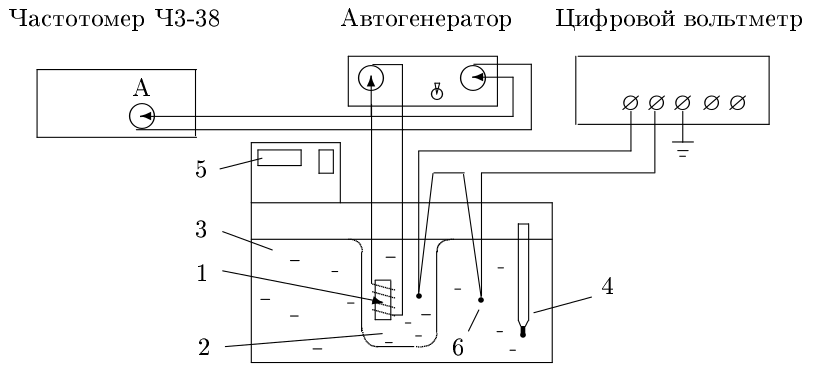
\includegraphics[width = 14cm]{facility}}
	\caption{Схема установки}
	\label{fig:image}
\end{figure}

При $T \rightarrow 0$ тепловое движение все меньше препятствует магнитным моментам атомовориентироваться в одном направлении при действии сколь угодно малого внешнего поля, в связи с чем $\chi$ неограниченно возрастает. В ферромагнетиках это происходит при понижении температуры не до 0, а до температуры Кюри $\Theta$. Оказывается, для ферромагнетиков закон Кюри должен быть заменен заоном Кюри-Вейсса:
$$
	\chi \sim \frac{1}{T - \Theta_p},
$$
\noindent где $\Theta_p$ - температура, близкая к $\Theta$.

В данной работе изучается зависимость $\chi(T)$ гадолиния, так как его точка Кюри лежит в интервале комнатных температур.

\vspace{1cm}
\textbf{Экспериментальная установка:} схема приведена на рисунке. Рабочий образец из гадолиния расположен внутри пустотелой катушки самоиндукции, входящей в состав колебательного контура, входящего в состав LC-автогенератора. Гадолиний - хороший проводник электрического тока, а рабочая частота генератора достаточно велика, поэтому для уменьшения вихревых токов образец изготовлен из мелких кусочков размером около 0.5 мм. Катушка 1 с образцом помещена в стеклянный сосуд 2, залитый трансформаторным маслом, предохраняющим образец от окисления и способствующим ухудшению контакта между кусочками образца, а также улучшающим тепловой контакт между образцом и жидкостью 3 в термостате. Термометр 4 используется для определения температуры термостата. 

Магнитную восприимчивость определяем по изменению самоиндукции катушки. Обозначив через $L$ самоиндукцию катушки с образцом, $L_0$ - без образца, получим 
$$
	(L - L_0) \sim \chi
$$
При изменении самоиндукции образа изменяется период колебаний автогенератора:
$$
	\tau = 2\pi\sqrt{LC},
$$
\noindent где $C$ - емкость контура. Период колебаний в отсутствие образца определяется самоиндукцией пустой катушки:
$$
	\tau_0 = 2\pi\sqrt{L_0C}
$$

Отсюда получим:
$$
	(L - L_0) \sim (\tau^2 - \tau_0^2)
$$
\noindent или
$$
	\chi \sim (\tau^2 - \tau_0^2)
$$

Отсюда видно:
$$
	(T - \Theta_p) \sim \frac{1}{(\tau^2 - \tau_0^2)}
$$

\vspace{1cm}
\textbf{Ход работы.} 

Первым делом определим допустимое ЭДС термопары, при котором разность температур образца и воды $\Delta T$ не более 0.5К, зная, что постоянная термопары 
$k = 24\frac{\text{град}}{\text{мВ}}$:
$$
	\varepsilon = \frac{\Delta T}{k} = 0.02~\text{мВ}
$$

Указанное на установке время $\tau_0 = 9.045$ мкс.

\vspace{1cm}
Теперь снимем зависимость $\tau(T)$:

\begin{center}
\begin{tabular}{|c|c|c|c|c|c|c|c|c|c|c|c|c|}
\hline
$T$, $^\circ C$		&	$\tau$, мкс		&	$1/(\tau^2 - \tau_0^2)$, $10^9/c^2$	&	$\sigma_{1/(\tau^2 - \tau_0^2)}$, $10^9/c^2$	\\
\hline
14.0				&	10.776			&	29.15									&	0.02											\\
\hline
16.0				&	10.677			&	31.07									&	0.02											\\
\hline
18.0				&	10.491			&	35.40									&	0.03											\\
\hline
20.0				&	10.191			&	45.36									&	0.04											\\
\hline
22.0				&	9.787			&	71.56									&	0.10											\\
\hline
24.0				&	9.530			&	111.0									&	0.2												\\
\hline
26.0				&	9.393			&	155.9									&	0.5												\\
\hline
28.0				&	9.324			&	195.1									&	0.7												\\
\hline
30.0				&	9.281			&	231.2									&	1.0												\\
\hline
32.0				&	9.244			&	274.8									&	1.4												\\
\hline
34.0				&	9.220			&	312.9									&	1.8												\\
\hline
36.0				&	9.201			&	351										&	2												\\
\hline
38.0				&	9.187			&	386										&	3												\\
\hline
40.0				&	9.176			&	419										&	3												\\
\hline
\end{tabular}
\end{center}


И построим график зависимости $T(1/(\tau^2 - \tau_0^2))$:

\vspace{0.5cm}
\begin{tikzpicture}
\begin{axis}[
	height = 10cm,
	width  = 15cm,
	every axis y label/.style={at = {(ticklabel cs: 0.5)}, rotate = 90, anchor = near ticklabel},
	xlabel = {$T, ^\circ C$},
	ylabel = {$\frac{1}{(\tau^2 - \tau_0^2)}, c\cdot 10^{12}$},
	grid   = major,
	ymin   = 0,
	xmin   = 12
]
\addplot+[
	only marks,
	error bars/.cd, 
	y dir = both, y explicit,
	x dir = both, x explicit,
	]
coordinates{
	(14, 0.029)		+-	(0.3, 0)
	(16, 0.031)		+-	(0.3, 0)
	(18, 0.035)		+-	(0.3, 0)
	(20, 0.045)		+-	(0.3, 0)
	(22, 0.072)		+-	(0.3, 0)
	(24, 0.111)		+-	(0.3, 0)
	(26, 0.156)		+-	(0.3, 0)
	(28, 0.195)		+-	(0.3, 0)
	(30, 0.231)		+-	(0.3, 0)
	(32, 0.275)		+-	(0.3, 0)
	(34, 0.313)		+-	(0.3, 0)
	(36, 0.351)		+-	(0.3, 0.002)
	(38, 0.386)		+-	(0.3, 0.003)
	(40, 0.419)		+-	(0.3, 0.003)
};

\addplot+[
	smooth,
	mark = none,
	blue
	]
coordinates{
	(14, 0.029)
	(16, 0.031)
	(18, 0.035)
	(20, 0.045)
	(22, 0.072)	% 5
	(24, 0.108)
	(26, 0.153)
	(28, 0.195)
	(30, 0.235)
	(32, 0.275)
	(34, 0.313)
	(36, 0.351)
	(38, 0.386)
	(40, 0.419)	
};

\addplot [mark = none]
coordinates{
	(18.2, 0)
	(40  , 0.426018)
};

\end{axis}
\end{tikzpicture}

Для оценки погрешности отметим, что погрешность $T$ можно принять равной $0.3~^\circ C$, так как мы дожидались, чтобы температура образца и воды в термостате отличалась не более, чем на 0.1 $^\circ C$, чему соответствуют показания вольтметра 10 мкВ (0.010 мВ $\cdot$ $24\frac{\text{град}}{\text{мВ}}$). Погрешностью определения температуры при помощи термометра, установленного на термостате, можно пренебречь. Погрешность же частоты возьмем равной 1 нс, так как следующий разряд на приборе колебался, а этот показывал постоянное значение.

Теперь определим парамагнитную точку Кюри $\Theta_p$ гадолиния, экстраполируя прямую. Видно, что полученное значение будет равно 18 $^\circ C$. При этом можем считать 
$\Theta_p = f(T, \tau)$, тогда приборную погрешность $\sigma_{\text{приб}} \approx \sigma_T = 0.3 K$. Из МНК можно оценить погрешность случайную: 
$\sigma_{\text{случ}} \approx 0.2 K$. Теперь можно найти полную погрешность по формуле
$$
	\sigma = \sqrt{\sigma_{\text{случ}}^2 + \sigma_{\text{приб}}^2} = 0.4 K
$$

Окончательно получим:
$$
	\boxed{\Theta_p = (18.0 \pm 0.4)~^\circ C}
$$
Табличное значение $\Theta_{p~\text{табл}} = 19 ^\circ C$, что с хорошей точностью согласуется с полученным в работе значением.

\vspace{1cm}
Таким образом, в данной лабораторной работе мы изучили температурную зависимость магнитной восприимчисвости гадолиния в диапазоне температур, близком к точке Кюри, а также определили значение парамагнитной точки Кюри $\Theta_p$ гадолиния. 






\end{document}